% Created 2026-04-10 Fri 17:25
% Intended LaTeX compiler: pdflatex
\documentclass[11pt]{article}
\usepackage[utf8]{inputenc}
\usepackage[T1]{fontenc}
\usepackage{graphicx}
\usepackage{longtable}
\usepackage{wrapfig}
\usepackage{rotating}
\usepackage[normalem]{ulem}
\usepackage{amsmath}
\usepackage{amssymb}
\usepackage{capt-of}
\usepackage{hyperref}
\usepackage[left=0.75in,right=0.75in,top=1in,bottom=1in]{geometry}
\usepackage{enumitem}
\setlist[itemize]{itemsep=2pt, topsep=4pt}
\author{Ben Heinze}
\date{\today}
\title{Data-Driven Model Structure Notes}
\hypersetup{
 pdfauthor={Ben Heinze},
 pdftitle={Data-Driven Model Structure Notes},
 pdfkeywords={},
 pdfsubject={},
 pdfcreator={Emacs 29.3 (Org mode 9.6.15)}, 
 pdflang={English}}
\begin{document}

\maketitle

\section{Question 1.}
\label{sec:orgea9a029}

Weight only needs the single subscript \(i\) because that is going to remain constant through each sweat measurement, so they only need to account for it on the subject level. The no-tattoo indicator, on the other hand, will change despite the subject being the same, so this is on the observation level.

\section{Question 2.}
\label{sec:org8aed758}

If the classmate used \(age_{ij}\) despite it being measured one per subject, at the observation level, \emph{modeldiagramR} uses data to generate a corrected model by creating a model diagram based on the data, which would make this student's mistake clearly visible. 


\section{Question 3.}
\label{sec:org5d4c5cc}

I'd use the LearnVizLMM package to check the model diagram fro lab 7 before cleaning and wrangling the data because it doesn't require the data or a model object to draw the diagram.


\section{Question 4.1}
\label{sec:org80a4671}

Measurement structure:

\begin{center}
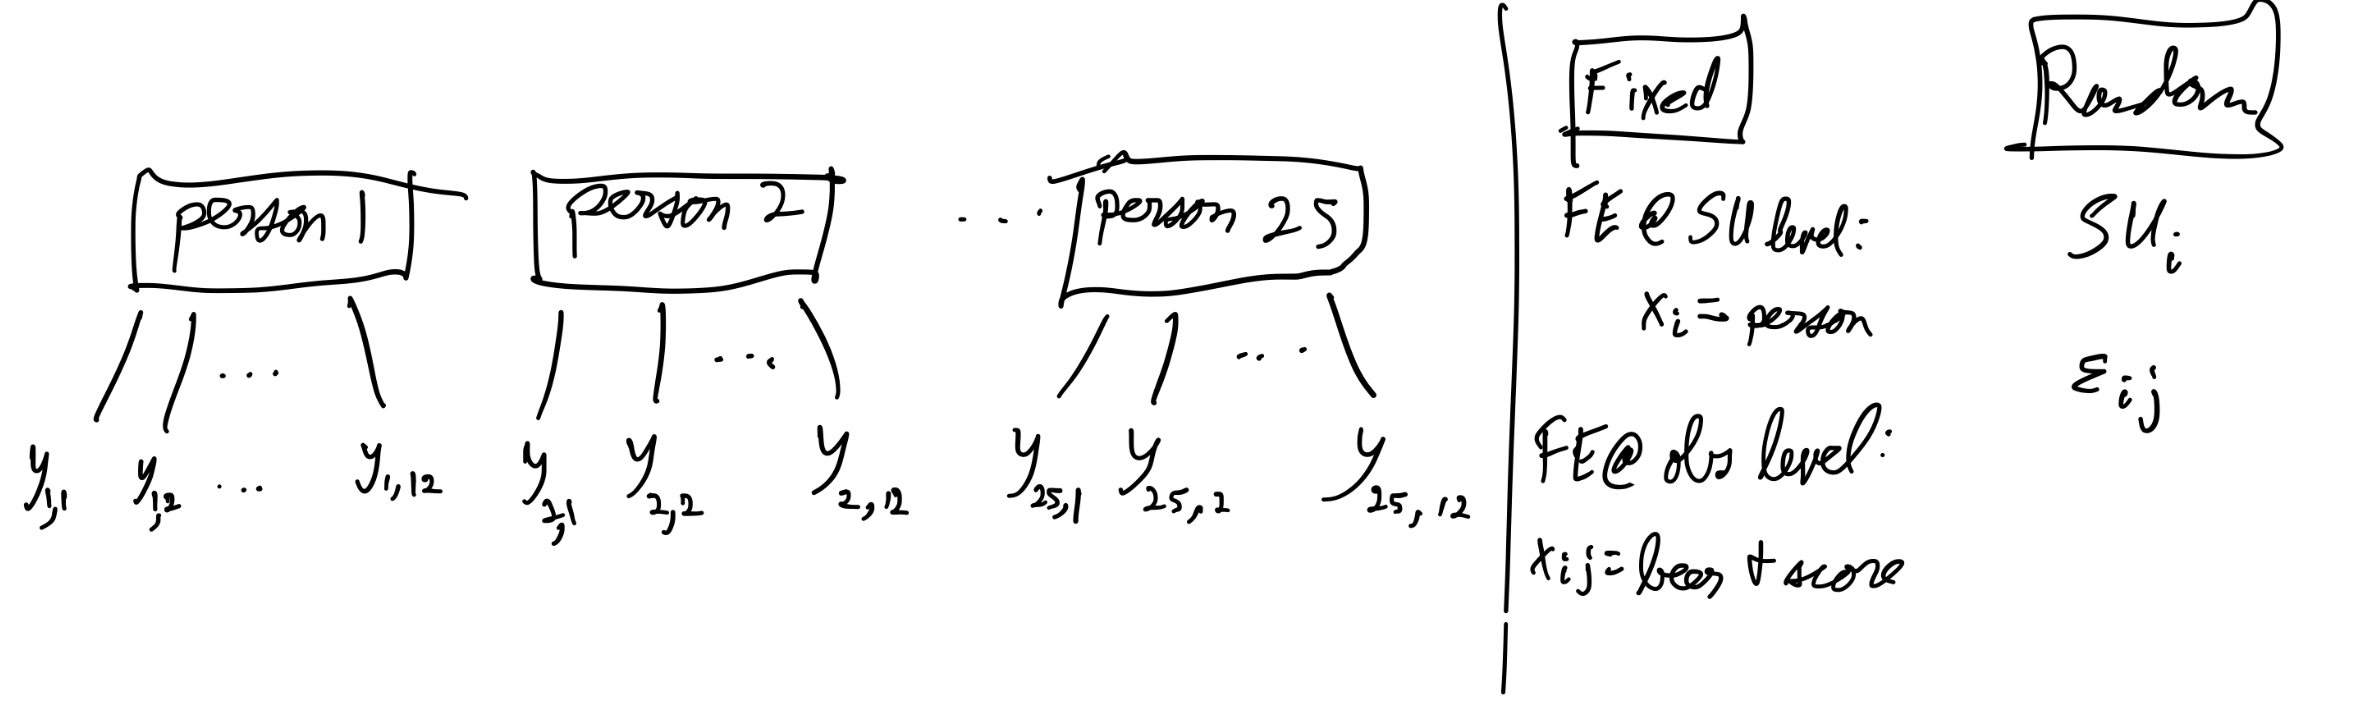
\includegraphics[width=.9\linewidth]{IMG_0038.jpg}
\end{center}

\begin{itemize}
\item fixed effects column:
\begin{itemize}
\item people @SU level (x\textsubscript{i})
\item Time they took quiz, liters of beer consumed @obs level (x\textsubscript{ij})
\end{itemize}
\item random effects column: SU\textsubscript{i}, \(\epsilon\)\textsubscript{ij}
\item i = 1-25 (index people)
\item j = 1-12, (index observation within people (number of tests taken))
\end{itemize}


Theoretical model:
\(\text{IQScore}_{ij} = \mu_{ij} + Person_{i} + \epsilon_{ij}\)

\(\mu_{ij} = \beta_0 + \beta_1 I_{test 2} + \ldots + \beta_11 I_{test 12} + \beta_{13} \text{beer_liters}\)
\[ SU_{i} \sim \mathcal{N} (0, \sigma^2_{person}) \]
\(\epsilon_{ij} \sim \mathcal{N} (0, \sigma^2)\)


Model params: 
\(\beta_0\): expected IQ for someone who doesn't drink
\(\beta_i\) = the change in intercept for test i compared to baseline
\(\beta_{13}\) = the change in intercept compared to baseline given the liter of beer they drank in the last two weeks.




\subsection{Subproblem 2.}
\label{sec:org3b8fc86}


\begin{center}
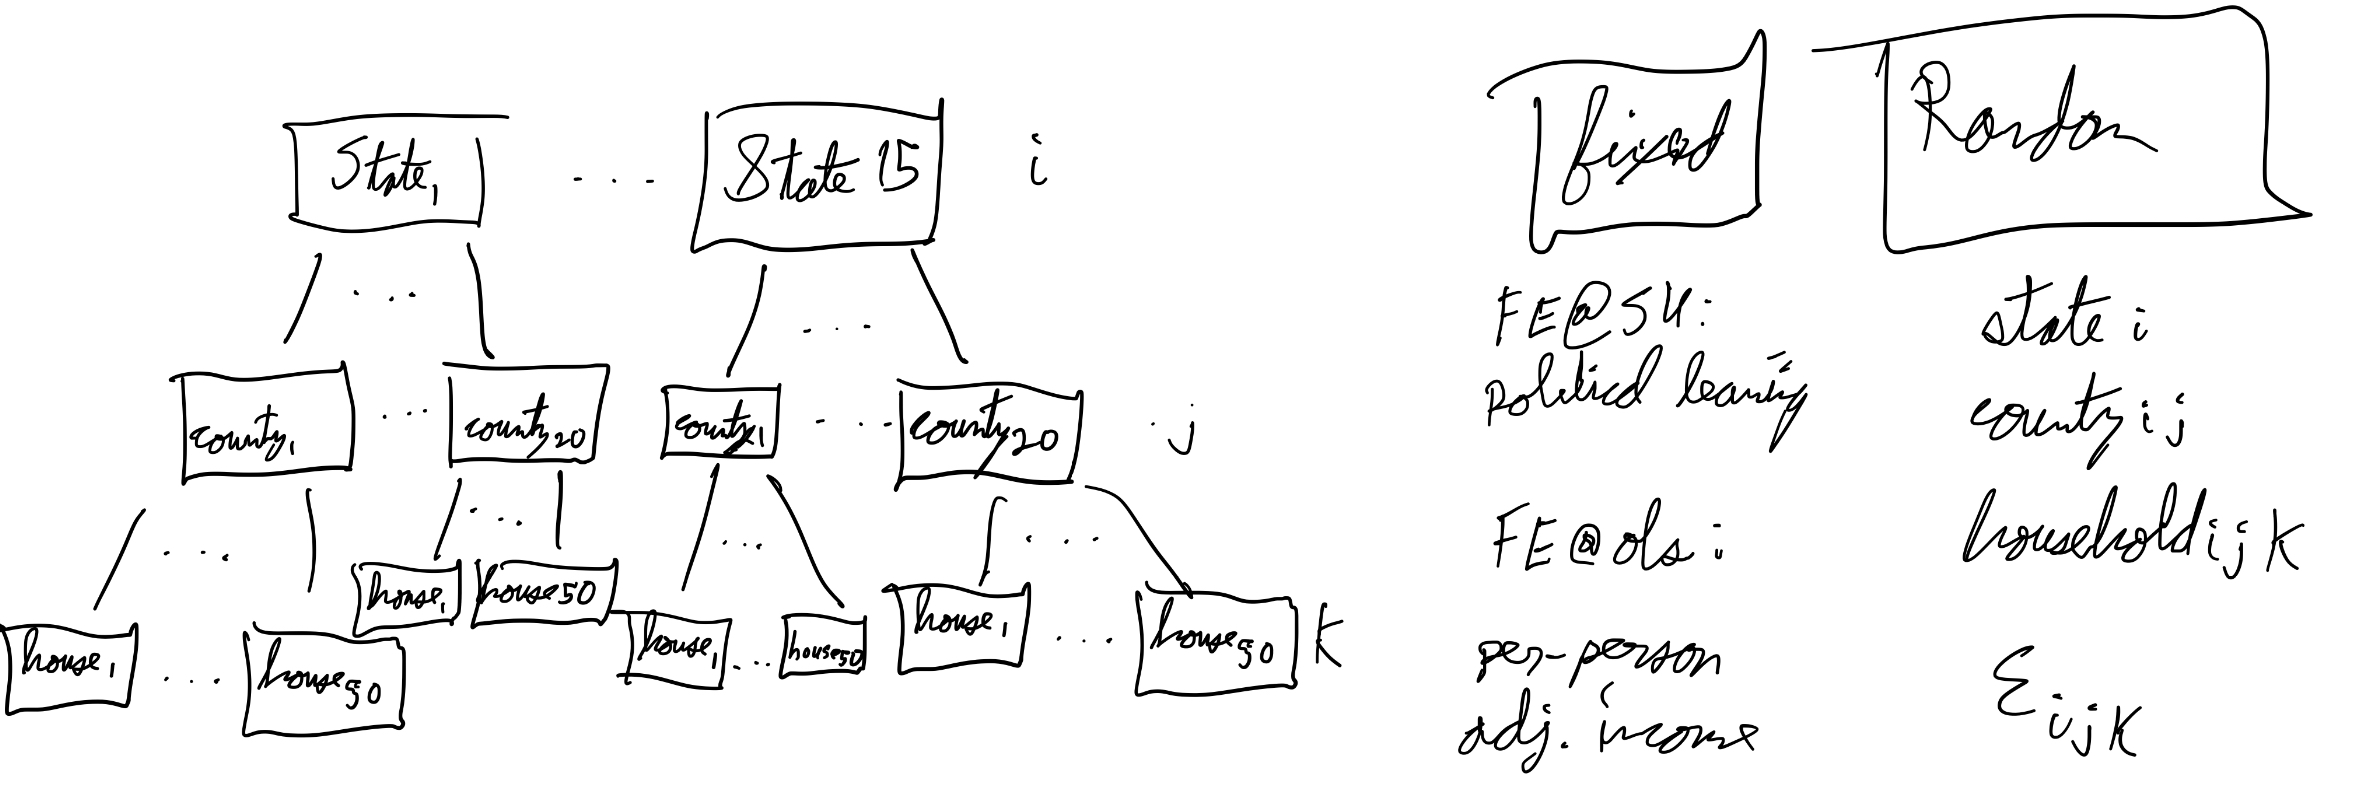
\includegraphics[width=.9\linewidth]{10456.jpg}
\end{center}


\begin{itemize}
\item i = 1-15 (index state)
\item j = 1-20 (index county)
\item k = 1-50 (index households)
\end{itemize}


Theoretical model:
\(diff_{ijk}= \mu_{ijk} + state_i + county_{ij} + household_{ijk} + \epsilon_{ijk}\)
\(\text{Diff_{ij}} = \mu_{ijk} + State_{i} + county_{ij} + household_{ijk} + \epsilon_{ijk}\)
\(\mu_{ijk} = \beta_0 + \beta_1 \text{per person adj income}} + \beta_2 I_{right_leaning} + \beta_3 \text{youngest}\)

\(state_{i} \sim \mathcal{N} (0, \sigma^2_{state})}\)
\(county_{ij} \sim \mathcal{N} (0, \sigma^2_{state})}\)
\(household_{ijk} \sim \mathcal{N} (0, \sigma^2_{state})}\)
\(\epsilon_{ij} \sim \mathcal{N} (0, \sigma^2)\)

Model params:
\(\beta_0\): mean adjusted household income for left-leaning if youngest per-person-adj income is zero and youngest age in household is zero
\(\beta_1\): how the intercept changes with the inclusion of per-person-adjusted-income compared to baseline
\(\beta_2\): how the intercept of baseline changes based on whether the county was right-leaning or not
\(\beta_3\) how the intercept of baseline changes based on age of the youngest person in the household
\end{document}
